% Neural network diagram
% Made with Xematics. Positions are in px (1 px = 0.75 pt), as in the SVG export.
\documentclass[tikz, border=4pt]{standalone}
\definecolor{xm1}{HTML}{15191F}
\definecolor{xm2}{HTML}{9AA3AE}
\definecolor{xm3}{HTML}{56B4E9}
\definecolor{xm4}{HTML}{9FD4F3}
\definecolor{xm5}{HTML}{2B313B}
\definecolor{xm6}{HTML}{E8EAED}
\definecolor{xm7}{HTML}{E69F00}
\definecolor{xm8}{HTML}{F3C45C}
\begin{document}
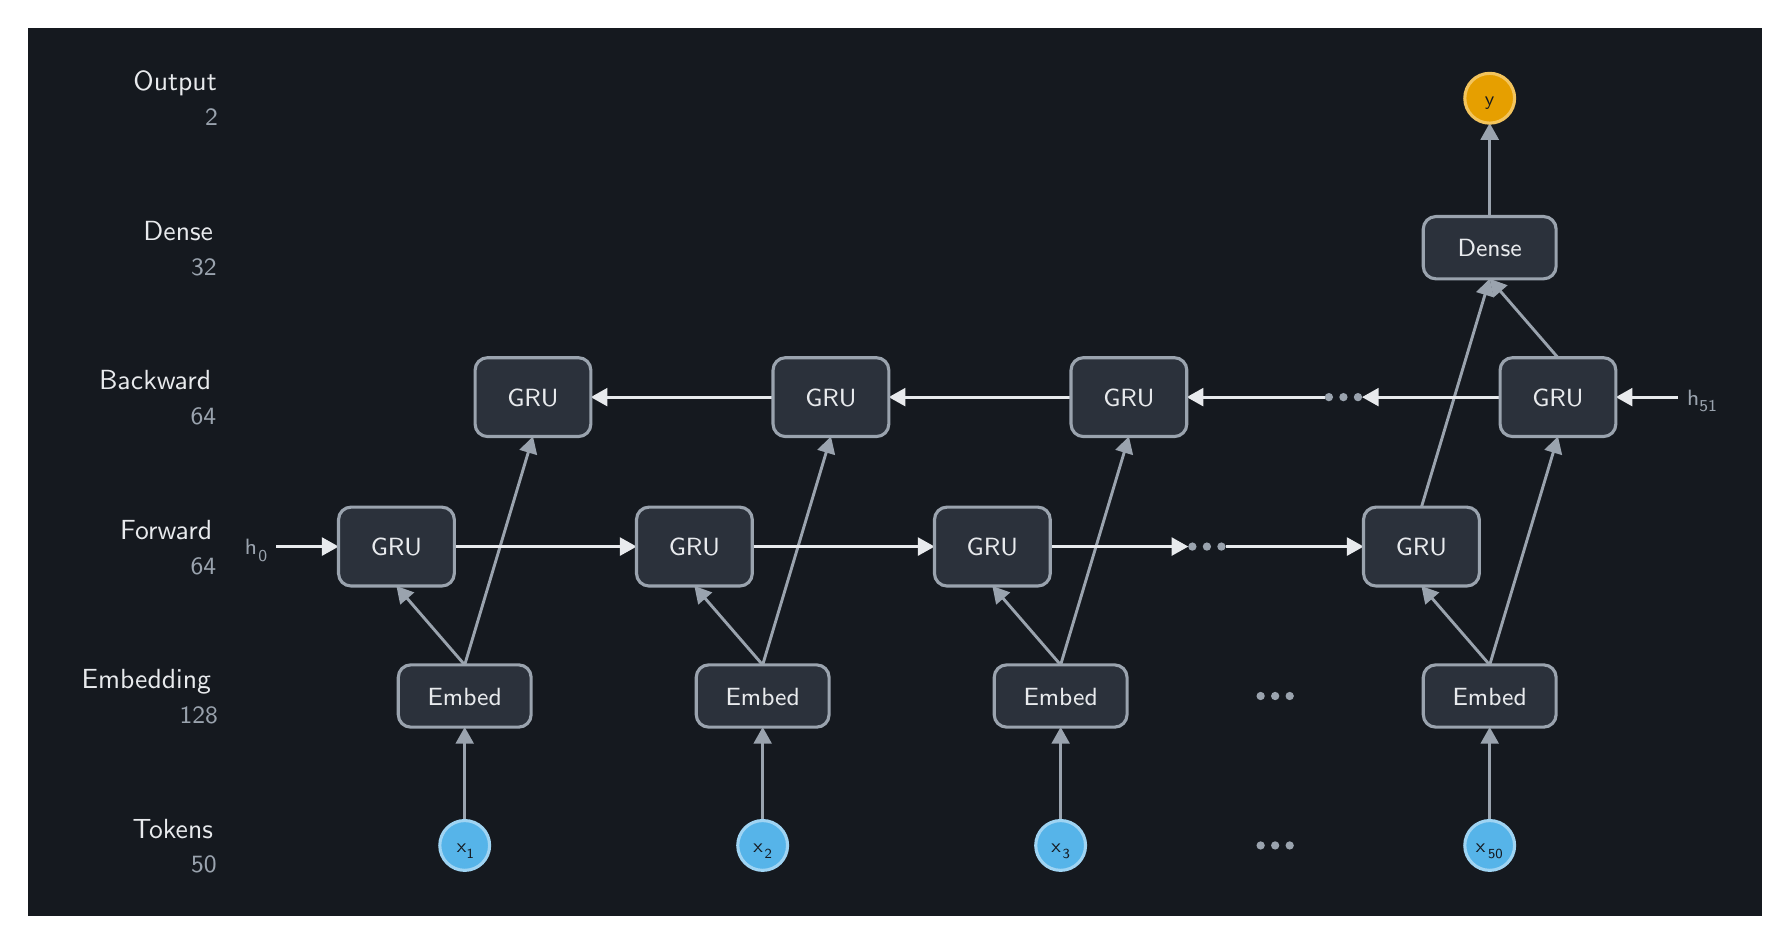
\begin{tikzpicture}[x=0.75pt, y=-0.75pt]
  \tikzset{
    xm arrow d6rgep/.style={draw=xm2, line width=1.05pt},
    xm arrow 14mtdps/.style={fill=xm2, line join=round},
    xm node 1gy69v8/.style={fill=xm3, draw=xm4, line width=1.13pt},
    xm text xm1/.style={text=xm1, inner sep=0},
    xm circle 1myn5oj/.style={fill=xm2},
    xm box 1mcw9mt/.style={fill=xm5, draw=xm2, line width=1.13pt, rounded corners=4.5pt},
    xm text xm6/.style={text=xm6, inner sep=0},
    xm state 1l69f7x/.style={draw=xm6, line width=1.05pt},
    xm state 19pejvw/.style={fill=xm6, line join=round},
    xm text xm2/.style={text=xm2, inner sep=0},
    xm node qnid0s/.style={fill=xm7, draw=xm8, line width=1.13pt},
  }
  \fill[xm1] (0,0) rectangle (835.61,428);
  % Diagram
  \path[xm arrow d6rgep] (210.56,382) -- (210.56,344);
  \path[xm arrow 14mtdps] (210.56,337) -- (215.06,345) -- (206.06,345) -- cycle;
  \path[xm arrow d6rgep] (354.12,382) -- (354.12,344);
  \path[xm arrow 14mtdps] (354.12,337) -- (358.62,345) -- (349.62,345) -- cycle;
  \path[xm arrow d6rgep] (497.68,382) -- (497.68,344);
  \path[xm arrow 14mtdps] (497.68,337) -- (502.18,345) -- (493.18,345) -- cycle;
  \path[xm arrow d6rgep] (704.4,382) -- (704.4,344);
  \path[xm arrow 14mtdps] (704.4,337) -- (708.9,345) -- (699.9,345) -- cycle;
  \path[xm arrow d6rgep] (210.56,307) -- (182.25,274.29);
  \path[xm arrow 14mtdps] (177.67,269) -- (186.31,272.1) -- (179.5,277.99) -- cycle;
  \path[xm arrow d6rgep] (210.56,307) -- (241.45,203.71);
  \path[xm arrow 14mtdps] (243.45,197) -- (245.47,205.95) -- (236.85,203.38) -- cycle;
  \path[xm arrow d6rgep] (354.12,307) -- (325.81,274.29);
  \path[xm arrow 14mtdps] (321.23,269) -- (329.87,272.1) -- (323.06,277.99) -- cycle;
  \path[xm arrow d6rgep] (354.12,307) -- (385,203.71);
  \path[xm arrow 14mtdps] (387.01,197) -- (389.03,205.95) -- (380.41,203.38) -- cycle;
  \path[xm arrow d6rgep] (497.68,307) -- (469.37,274.29);
  \path[xm arrow 14mtdps] (464.79,269) -- (473.43,272.1) -- (466.62,277.99) -- cycle;
  \path[xm arrow d6rgep] (497.68,307) -- (528.56,203.71);
  \path[xm arrow 14mtdps] (530.57,197) -- (532.59,205.95) -- (523.97,203.38) -- cycle;
  \path[xm arrow d6rgep] (704.4,307) -- (676.09,274.29);
  \path[xm arrow 14mtdps] (671.51,269) -- (680.15,272.1) -- (673.35,277.99) -- cycle;
  \path[xm arrow d6rgep] (704.4,307) -- (735.29,203.71);
  \path[xm arrow 14mtdps] (737.29,197) -- (739.31,205.95) -- (730.69,203.38) -- cycle;
  \path[xm arrow d6rgep] (671.51,231) -- (702.4,127.71);
  \path[xm arrow 14mtdps] (704.4,121) -- (706.42,129.95) -- (697.8,127.38) -- cycle;
  \path[xm arrow d6rgep] (737.29,159) -- (708.98,126.29);
  \path[xm arrow 14mtdps] (704.4,121) -- (713.04,124.1) -- (706.24,129.99) -- cycle;
  \path[xm arrow d6rgep] (704.4,91) -- (704.4,53);
  \path[xm arrow 14mtdps] (704.4,46) -- (708.9,54) -- (699.9,54) -- cycle;
  \path[xm node 1gy69v8] (210.56,394) circle[radius=12];
  \node[xm text xm1, font=\sffamily\fontsize{7.5}{9}\selectfont, anchor=base] at (209.1,397.64) {x};
  \node[xm text xm1, font=\sffamily\fontsize{5.4}{6.48}\selectfont, anchor=base] at (213.29,400.44) {1};
  \path[xm node 1gy69v8] (354.12,394) circle[radius=12];
  \node[xm text xm1, font=\sffamily\fontsize{7.5}{9}\selectfont, anchor=base] at (351.92,397.64) {x};
  \node[xm text xm1, font=\sffamily\fontsize{5.4}{6.48}\selectfont, anchor=base] at (356.85,400.44) {2};
  \path[xm node 1gy69v8] (497.68,394) circle[radius=12];
  \node[xm text xm1, font=\sffamily\fontsize{7.5}{9}\selectfont, anchor=base] at (495.45,397.64) {x};
  \node[xm text xm1, font=\sffamily\fontsize{5.4}{6.48}\selectfont, anchor=base] at (500.41,400.44) {3};
  \path[xm circle 1myn5oj] (594.04,394) circle[radius=2];
  \path[xm circle 1myn5oj] (601.04,394) circle[radius=2];
  \path[xm circle 1myn5oj] (608.04,394) circle[radius=2];
  \path[xm node 1gy69v8] (704.4,394) circle[radius=12];
  \node[xm text xm1, font=\sffamily\fontsize{7.5}{9}\selectfont, anchor=base] at (700,397.64) {x};
  \node[xm text xm1, font=\sffamily\fontsize{5.4}{6.48}\selectfont, anchor=base] at (707.13,400.44) {50};
  \path[xm box 1mcw9mt] (178.56,307) rectangle ++(64,30);
  \node[xm text xm6, font=\sffamily\fontsize{9}{10.8}\selectfont, anchor=base] at (210.56,326.37) {Embed};
  \path[xm box 1mcw9mt] (322.12,307) rectangle ++(64,30);
  \node[xm text xm6, font=\sffamily\fontsize{9}{10.8}\selectfont, anchor=base] at (354.12,326.37) {Embed};
  \path[xm box 1mcw9mt] (465.68,307) rectangle ++(64,30);
  \node[xm text xm6, font=\sffamily\fontsize{9}{10.8}\selectfont, anchor=base] at (497.68,326.37) {Embed};
  \path[xm circle 1myn5oj] (594.04,322) circle[radius=2];
  \path[xm circle 1myn5oj] (601.04,322) circle[radius=2];
  \path[xm circle 1myn5oj] (608.04,322) circle[radius=2];
  \path[xm box 1mcw9mt] (672.4,307) rectangle ++(64,30);
  \node[xm text xm6, font=\sffamily\fontsize{9}{10.8}\selectfont, anchor=base] at (704.4,326.37) {Embed};
  \path[xm state 1l69f7x] (205.56,250) -- (286.34,250);
  \path[xm state 19pejvw] (293.34,250) -- (285.34,254.5) -- (285.34,245.5) -- cycle;
  \path[xm state 1l69f7x] (349.12,250) -- (429.9,250);
  \path[xm state 19pejvw] (436.9,250) -- (428.9,254.5) -- (428.9,245.5) -- cycle;
  \path[xm state 1l69f7x] (492.68,250) -- (552.15,250);
  \path[xm state 19pejvw] (559.15,250) -- (551.15,254.5) -- (551.15,245.5) -- cycle;
  \path[xm state 1l69f7x] (577.15,250) -- (636.62,250);
  \path[xm state 19pejvw] (643.62,250) -- (635.62,254.5) -- (635.62,245.5) -- cycle;
  \path[xm state 1l69f7x] (119.78,250) -- (142.78,250);
  \path[xm state 19pejvw] (149.78,250) -- (141.78,254.5) -- (141.78,245.5) -- cycle;
  \node[xm text xm2, font=\sffamily\fontsize{8.25}{9.9}\selectfont, anchor=base] at (107.53,254) {h};
  \node[xm text xm2, font=\sffamily\fontsize{5.94}{7.13}\selectfont, anchor=base] at (113.28,257.08) {0};
  \path[xm box 1mcw9mt] (149.78,231) rectangle ++(55.78,38);
  \node[xm text xm6, font=\sffamily\fontsize{9}{10.8}\selectfont, anchor=base] at (177.67,254.37) {GRU};
  \path[xm box 1mcw9mt] (293.34,231) rectangle ++(55.78,38);
  \node[xm text xm6, font=\sffamily\fontsize{9}{10.8}\selectfont, anchor=base] at (321.23,254.37) {GRU};
  \path[xm box 1mcw9mt] (436.9,231) rectangle ++(55.78,38);
  \node[xm text xm6, font=\sffamily\fontsize{9}{10.8}\selectfont, anchor=base] at (464.79,254.37) {GRU};
  \path[xm circle 1myn5oj] (561.15,250) circle[radius=2];
  \path[xm circle 1myn5oj] (568.15,250) circle[radius=2];
  \path[xm circle 1myn5oj] (575.15,250) circle[radius=2];
  \path[xm box 1mcw9mt] (643.62,231) rectangle ++(55.78,38);
  \node[xm text xm6, font=\sffamily\fontsize{9}{10.8}\selectfont, anchor=base] at (671.51,254.37) {GRU};
  \path[xm state 1l69f7x] (359.12,178) -- (278.34,178);
  \path[xm state 19pejvw] (271.34,178) -- (279.34,173.5) -- (279.34,182.5) -- cycle;
  \path[xm state 1l69f7x] (502.68,178) -- (421.9,178);
  \path[xm state 19pejvw] (414.9,178) -- (422.9,173.5) -- (422.9,182.5) -- cycle;
  \path[xm state 1l69f7x] (624.93,178) -- (565.46,178);
  \path[xm state 19pejvw] (558.46,178) -- (566.46,173.5) -- (566.46,182.5) -- cycle;
  \path[xm state 1l69f7x] (709.4,178) -- (649.93,178);
  \path[xm state 19pejvw] (642.93,178) -- (650.93,173.5) -- (650.93,182.5) -- cycle;
  \path[xm state 1l69f7x] (795.18,178) -- (772.18,178);
  \path[xm state 19pejvw] (765.18,178) -- (773.18,173.5) -- (773.18,182.5) -- cycle;
  \node[xm text xm2, font=\sffamily\fontsize{8.25}{9.9}\selectfont, anchor=base] at (802.43,182) {h};
  \node[xm text xm2, font=\sffamily\fontsize{5.94}{7.13}\selectfont, anchor=base] at (809.65,185.08) {51};
  \path[xm box 1mcw9mt] (215.56,159) rectangle ++(55.78,38);
  \node[xm text xm6, font=\sffamily\fontsize{9}{10.8}\selectfont, anchor=base] at (243.45,182.37) {GRU};
  \path[xm box 1mcw9mt] (359.12,159) rectangle ++(55.78,38);
  \node[xm text xm6, font=\sffamily\fontsize{9}{10.8}\selectfont, anchor=base] at (387.01,182.37) {GRU};
  \path[xm box 1mcw9mt] (502.68,159) rectangle ++(55.78,38);
  \node[xm text xm6, font=\sffamily\fontsize{9}{10.8}\selectfont, anchor=base] at (530.57,182.37) {GRU};
  \path[xm circle 1myn5oj] (626.93,178) circle[radius=2];
  \path[xm circle 1myn5oj] (633.93,178) circle[radius=2];
  \path[xm circle 1myn5oj] (640.93,178) circle[radius=2];
  \path[xm box 1mcw9mt] (709.4,159) rectangle ++(55.78,38);
  \node[xm text xm6, font=\sffamily\fontsize{9}{10.8}\selectfont, anchor=base] at (737.29,182.37) {GRU};
  \path[xm box 1mcw9mt] (672.4,91) rectangle ++(64,30);
  \node[xm text xm6, font=\sffamily\fontsize{9}{10.8}\selectfont, anchor=base] at (704.4,110.37) {Dense};
  \path[xm node qnid0s] (704.4,34) circle[radius=12];
  \node[xm text xm1, font=\sffamily\fontsize{7.5}{9}\selectfont, anchor=base] at (704.4,37.64) {y};
  \node[xm text xm6, font=\sffamily\fontsize{9.75}{11.7}\selectfont, anchor=base] at (69.9,390.47) {Tokens};
  \node[xm text xm2, font=\sffamily\fontsize{9}{10.8}\selectfont, anchor=base] at (84.94,407.23) {50};
  \node[xm text xm6, font=\sffamily\fontsize{9.75}{11.7}\selectfont, anchor=base] at (57.14,318.47) {Embedding};
  \node[xm text xm2, font=\sffamily\fontsize{9}{10.8}\selectfont, anchor=base] at (82.47,335.23) {128};
  \node[xm text xm6, font=\sffamily\fontsize{9.75}{11.7}\selectfont, anchor=base] at (66.71,246.47) {Forward};
  \node[xm text xm2, font=\sffamily\fontsize{9}{10.8}\selectfont, anchor=base] at (84.68,263.23) {64};
  \node[xm text xm6, font=\sffamily\fontsize{9.75}{11.7}\selectfont, anchor=base] at (61.45,174.47) {Backward};
  \node[xm text xm2, font=\sffamily\fontsize{9}{10.8}\selectfont, anchor=base] at (84.68,191.23) {64};
  \node[xm text xm6, font=\sffamily\fontsize{9.75}{11.7}\selectfont, anchor=base] at (72.54,102.47) {Dense};
  \node[xm text xm2, font=\sffamily\fontsize{9}{10.8}\selectfont, anchor=base] at (84.92,119.23) {32};
  \node[xm text xm6, font=\sffamily\fontsize{9.75}{11.7}\selectfont, anchor=base] at (71.04,30.47) {Output};
  \node[xm text xm2, font=\sffamily\fontsize{9}{10.8}\selectfont, anchor=base] at (88.62,47.23) {2};
\end{tikzpicture}
\end{document}
